\documentclass[10pt,twocolumn]{witseiepaper}

% All KJN's macros and goodies (some shameless borrowing from SPL)

\usepackage{KJN}
\usepackage{amsmath,amsfonts}
\usepackage{listings} 
\usepackage{tikz}
\usepackage{verbatim}
\usetikzlibrary{shapes.arrows}
\usetikzlibrary{shapes.geometric}
\usetikzlibrary{plotmarks}
\usetikzlibrary{matrix}
\usepackage{pgfplots}
\usepackage{circuitikz}
\usepackage{pdfpages}
\usepackage{placeins}
\usepackage{dblfloatfix}
\usepackage{graphicx}
\usepackage{caption}
\usepackage{subcaption}
\usepackage{url}
\makeatletter
\g@addto@macro{\UrlBreaks}{\UrlOrds}
\makeatother
\usepackage{cleveref}
\usepackage{color,soul}
\usepackage{float}

\pagestyle{plain}

%\addtolength{\oddsidemargin}{-.15in}
%\addtolength{\evensidemargin}{-.15in}
%\addtolength{\textwidth}{0.5in}

%%%%%%%%%%%%%%%%%%%%%%%%%%%%%%%%%%%%%%%%%%%%%%%%%%%
\begin{document}
	
	
\title{ELEN4012 - Cool project name here}
	
\author{Jared Ping (704447) \& Lara Timm (704157)
	\thanks{School of Electrical \& Information Engineering, University of the
			Witwatersrand, Private Bag 3, 2050, Johannesburg, South Africa}
}
	
%%%%%%%%%%%%%%%%%%%%%%%%%%%%%%%%%%%%%%%%%%%%%%%%%%%
\abstract{}
	
\keywords{}
	
\maketitle
%%%%%%%%%%%%%%%%%%%%%%%%%%%%%%%%%%%%%%%%%%%%%%%%%%%%
\section{INTRODUCTION}

%\textbf{THINGS THIS DOC NEEDS}
%\begin{itemize}
%	\item Circuit diagram
%	\item Ideas on how the housing will work
% ALGORITHMS
%	\item How we plan to program the arduinos (algorithm of operation)
%	\item How we plan to pass info between modules (algorithm of operation)
%	\item How we plan to display the info in the UI - maybe just programming platform and thoughts
%\end{itemize}

% GOOD PAPER FOR GENERAL SHIT - https://www.researchgate.net/profile/Carlo_Guarnieri_Calo_Carducci/publication/282855975_Design_of_a_Low_Cost_Multipurpose_Wireless_Sensor_Network/links/579e07e308ae6a2882f53965.pdf

%Have a badass introduction. Mention what IoT is 

\section{BACKGROUND AND CONTEXTUALISATION}
	The purpose of this section is to demonstrate techniques to identify and communicate parking bay availability. This process includes data acquisition and processing via a sensor module (with sensors, microcontroller (MCU), communication module and power supply), the actual deployment of the sensor module, wireless data communication, data management and data presentation. 

	\subsection{Hardware Choices} 
	% not sure if this section is too necessary - kinda just bullshitting, could be done concisely elsewhere
	
		\subsubsection{Microcontroller} $   $
		
			When choosing an MCU for an internet of things (IoT) system it is important to consider the MCU's power consumption, number and availability of I/O ports, how the module will interface with the sensors and how the sensor modules will communicate wirelessly with one another. Additional considerations are the ease of use of the module (how easy it is to interface with the hardware, ease of programming) and the size and expense of the MCU.
			
			% arduino has preexisting libraries for NRF24L01+ tranceiver as well as the HCSR04 Ultrasonic Sensor
			A popular, versatile and relatively inexpensive MCU platform is the Arduino Platform. Owing to their small size and reasonable price, the Arduino Nano V3 and Arduino Pro Mini were considered. Arduino devices are well documented, with a wide array of libraries, provide through extensive community support, existing to support a range of inexpensive sensor and communication modules. The Nano is advantageous over the Pro Mini due to its ease of programming, greater availability and lower current draw during normal operation due to an inefficient power regulator integrated circuit (IC) in the Pro Mini.

			%ESP board - stuff. NEEDS HELP
			An alternative to Arduino development boards are the ESP8266 based MCUs. A range of development boards based on the aforementioned microprocessor are commercially available. These boards designed to cater for low consumption requirements, such as the bare-bones ESP8266 MCU, through to intensive processing requirements, such as the dual core ESP32 MCU. The development boards come pre-built with a Wi-Fi module, among other communication modules, which negates the requirements of additional communication hardware~\cite{esp12e}.
			
		\subsubsection{Sensor} $   $
			
			The sensor chosen to detect vehicle presence in an open air parking lot should be tolerant of the environmental conditions in which it must operate. With large amounts of ambient light, varying light conditions, fluctuating temperatures and possible rain exposure the sensor should be raised from ground level, should not rely on light to detect vehicles and should not be significantly affected by changing temperatures. Considering also that the cost per unit should be as low as possible, connecting multiple sensors to a single MCU is a reasonable design choice.
			 
			This specification suggests the use of an ultrasonic sensor with special considerations for waterproofing. Ultrasonic sensors are accurate distance measurement sensors and enable, through software configuration, the type of object being detected to be ascertained and as such the number of false positives to be reduced.		
			
		\subsubsection{Communication} $   $

			The method of communication between the sensor nodes is a key design consideration as many options are available, each with their own benefits and trade-offs. A range of communication modules exist which are compatible with most common MCUs. These include Wi-Fi, RF, Bluetooth and NFC communication standards. The chosen mode of communication should be robust and reliable as to prevent data loss during transmission. Furthermore, the communication modules should be able to endure a range of outdoor weather conditions as well as obstructions which may exist between two modules.

			The solution should be designed to cater for a system that can be easily and efficiently scaled. This requires the abundant availability of channels within the chosen communication scheme to prevent bandwidth throttling within the sensor network. It is pivotal that an energy efficient communication scheme is utilised in that the power consumption of the communication modules provides an ideal transmission range. Power consumption is proportional to transmission range and a communication module with variable power modes would be ideal for a scalable and power efficient solution. Enabling line of sight between nodes to be achieved, where possible, would require less power as transmission does not need to occur trough any obstacles.
			%must be done in such a way that the system is scalable, NB as this project needs to prove concept
			%low power is good
			%range extended by making a 'line of sight' between the modules - lower power consumption is achieved.
			
		\subsubsection{Power Supply} $   $
			%Consider using a regulated sousrce such as a power bank, must be able to supply around 200 mA. Power - MCU, sensors, comm module. Power bank - cheap, readily available, charging and discharging circuitry problem presented when auto-off is enabled. Safety feature for when too little current is drawn. 
			%Source must be sustainable, want unit to have a long life, batteries must last long / be recharged / both.
			%NiMh batteries are cheap, rechargable, small size 
			When considering that the sensor network should be portable and self-sufficient, the power supply modules should be able to power the network independently. The sensor network requires supply modules which are well regulated and offer large capacity. Additionally, the modules should be renewable and affordable. Rechargeable batteries cater for this exact purpose.

			A range of rechargeable batteries exist which include lithium ion (Li-ion), lithium polymer (Li-Po) and nickel metal hydride (Ni-Mh) options. Li-ion batteries generally offer high capacity in 3.7 V multiples but are known to be quite dangerous when exposed to high temperature ranges~\cite{li-ion}. Li-Po batteries offer a large range of capacities in 3.7 V multiples but the price increases exponentially as capacity increases~\cite{li-po}. Ni-Mh batteries are versatile in offering a large range of capacities as well as a range of voltages~\cite{ni-mh}.

			The chosen supply will then need to be regulated to ensure stable operation of the sensor nodes as any fluctuation in supply may damage or prevent the sensor nodes from correctly functioning. To ensure the supplied voltage is at an expected level, the use of a boost converter could be utilised to step up the default supply voltage of the batteries.
	
	\subsection{Communication Technologies}
		\subsubsection{Wi-Fi}
			Wi-Fi is well known and easily accessible communication scheme in the IoT market. It's range will vary on a range of factors which include the specific IEEE 802.11 protocol which the module is utilising, the strength of the module's transmitter, and radio interference from the surrounding environment~\cite{802.11}. Low energy consumption modules require between 14~dBm (25~mW) to 19~dBm (79~mW) for typical transmission with a data rate of 72~Mbps~\cite{esp12e}. At maximum transmission power in an open environment, a maximum transmission distance of approximately 100~m is obtained~\cite{esp12e}. The ESP8266 Wi-Fi module allows four simultaneous client connections with unidirectional communication~\cite{esp12e}.

		\subsubsection{Bluetooth}
			Bluetooth is another well known communication scheme which is available within the IoT market. It utilises the IEEE 802.15.1 and there are multiple variants which offer differing combinations of low energy consumption, high data rates and long transmission distances~\cite{802.15.2}. Low energy consumption modules require a maximum of 3~dBm (2mW) for a typical transmission that can transmit a at a maximum range of approximately 150~m with a data rate of 0.23~Mbps~\cite{BLE112}. The long range variant offers a maximum transmission distance of approximately 450~m with a data rate of 0.23~Mbps with a transmission power requirement of 8~dBm (6~mW)~\cite{BLE112LR}. The number of simultaneous connections allowed varies per device, with the maximum amount being seven, with unidirectional communication~\cite{bluetooth-users}.

		\subsubsection{Radio Frequency}
			A range of RF-based transceivers exist which utilise different ISM bands. The NRF24 refers to a protocol utilised by Nordic Semiconductors in which they utilise the 2.4~GHz ISM band for RF communication~\cite{nrf24}. Nordic has produced a range of NRF24 based transceivers which have become prominent within the IoT market due to their low cost and adjustable power consumption. The nRF24L01+ transceiver, for example, offers a maximum transmission distance of approximately 100~m with a data rate of 0.25~Mbps with a transmission power requirement of 0~dBm (1~mW)~\cite{nrf24}. Furthermore, the data rate can be configured up to 2~Mbps and transmission power modes can be selected ranging down to -18~dBm (16~$\mu$W)~\cite{nrf24}. These transceivers facilitate 125 simultaneous connections with bidirectional communication~\cite{nrf24}.
			
			An alternative is the RFM69 transceiver, which offers similar operating characteristics to the NRF24-based transceivers but operates in the 433/868/915~Mhz ISM bands and supports up to 255 simultaneous connections~\cite{rfm69}. Naturally, the RFM69 transceiver exhibits marginally higher power requirements to sustain these capabilities and is higher priced than the NRF24-based transceivers~\cite{rfm69}.
	
	\subsection{Deployment Methodologies}
		The parking system is to be deployed in the 3rd, 4th and Postgraduate Parking lot near the Chamber of Mines building on the West Campus of Wits University. The designed system covers 72 parking spaces, with four sensors being monitored by each MCU. As such, 18 hardware modules need to be packaged and deployed. Figure~\ref{fig:deployment} shows the planned deployment layout. Considerations have been made for the module rigidity, resistance to environmental conditions, security and positioning.
		
		\begin{figure}
			\centering
			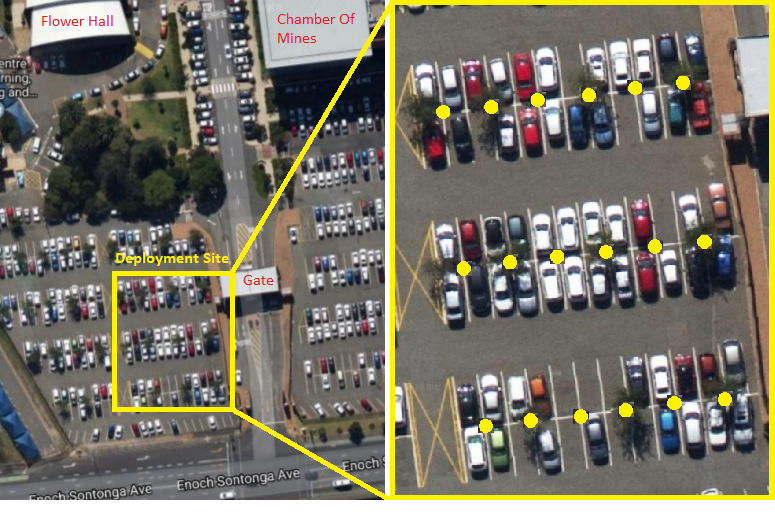
\includegraphics[width=1\columnwidth]{media/deploymentSite.png}
			\caption{Smart Parking deployment site (Google Maps Satellite View) and Module Placement Map}
			\raggedright
			\label{fig:deployment}
		\end{figure}
	
		%\subsubsection{Rigidity}
		It is obvious that the deployed hardware should be raised from ground level, not only to prevent the circuitry from being damaged by excessive water runoff, but also to provide the ultrasonic sensors with the best viewing angle and ensure that all shapes and sizes of vehicles are detected. The use of an ultrasonic sensor also provides challenges regarding waterproofing due to the nature of ultrasonic waves being impermeable to almost all materials. As such, there cannot be any barrier between the sensors and the cars being detected, requiring a runoff system that will keep this circuitry dry. 
		
		Raising the hardware requires that the sensor nodes are resilient to strong winds, and should not break if they are bumped by vehicles driving into or between parking spaces. In an attempt to keep costs to a minimum, a PVC stand is proposed that will be rigid, stable and provide the right topology to detect vehicles at average bumper height. A top and isometric view of the proposed stand is provided in Figure~\ref{fig:stand}. As an alternative, a traffic cone could be used to house the system, if an inexpensive yet rigid option can be sourced.
		
		\begin{figure}
			\centering
			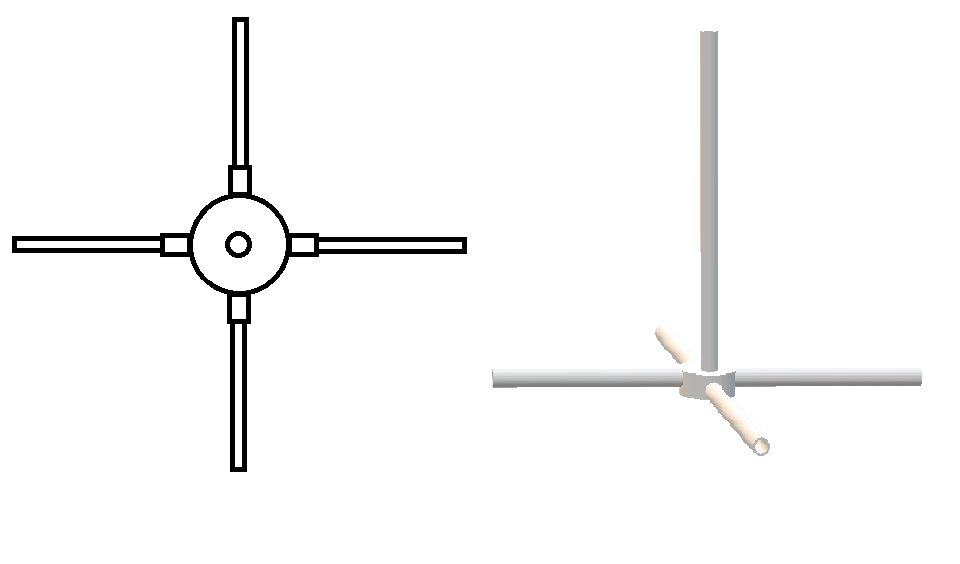
\includegraphics[width=1\columnwidth]{media/topIsoStand.png}
			\caption{Top (left) and Isometric (right) view of the proposed PVC stand}
			\raggedright
			\label{fig:stand}
		\end{figure}
	
	\subsection{Data Management}
		\subsubsection{Network Mesh}
			\begin{figure}
				\centering
				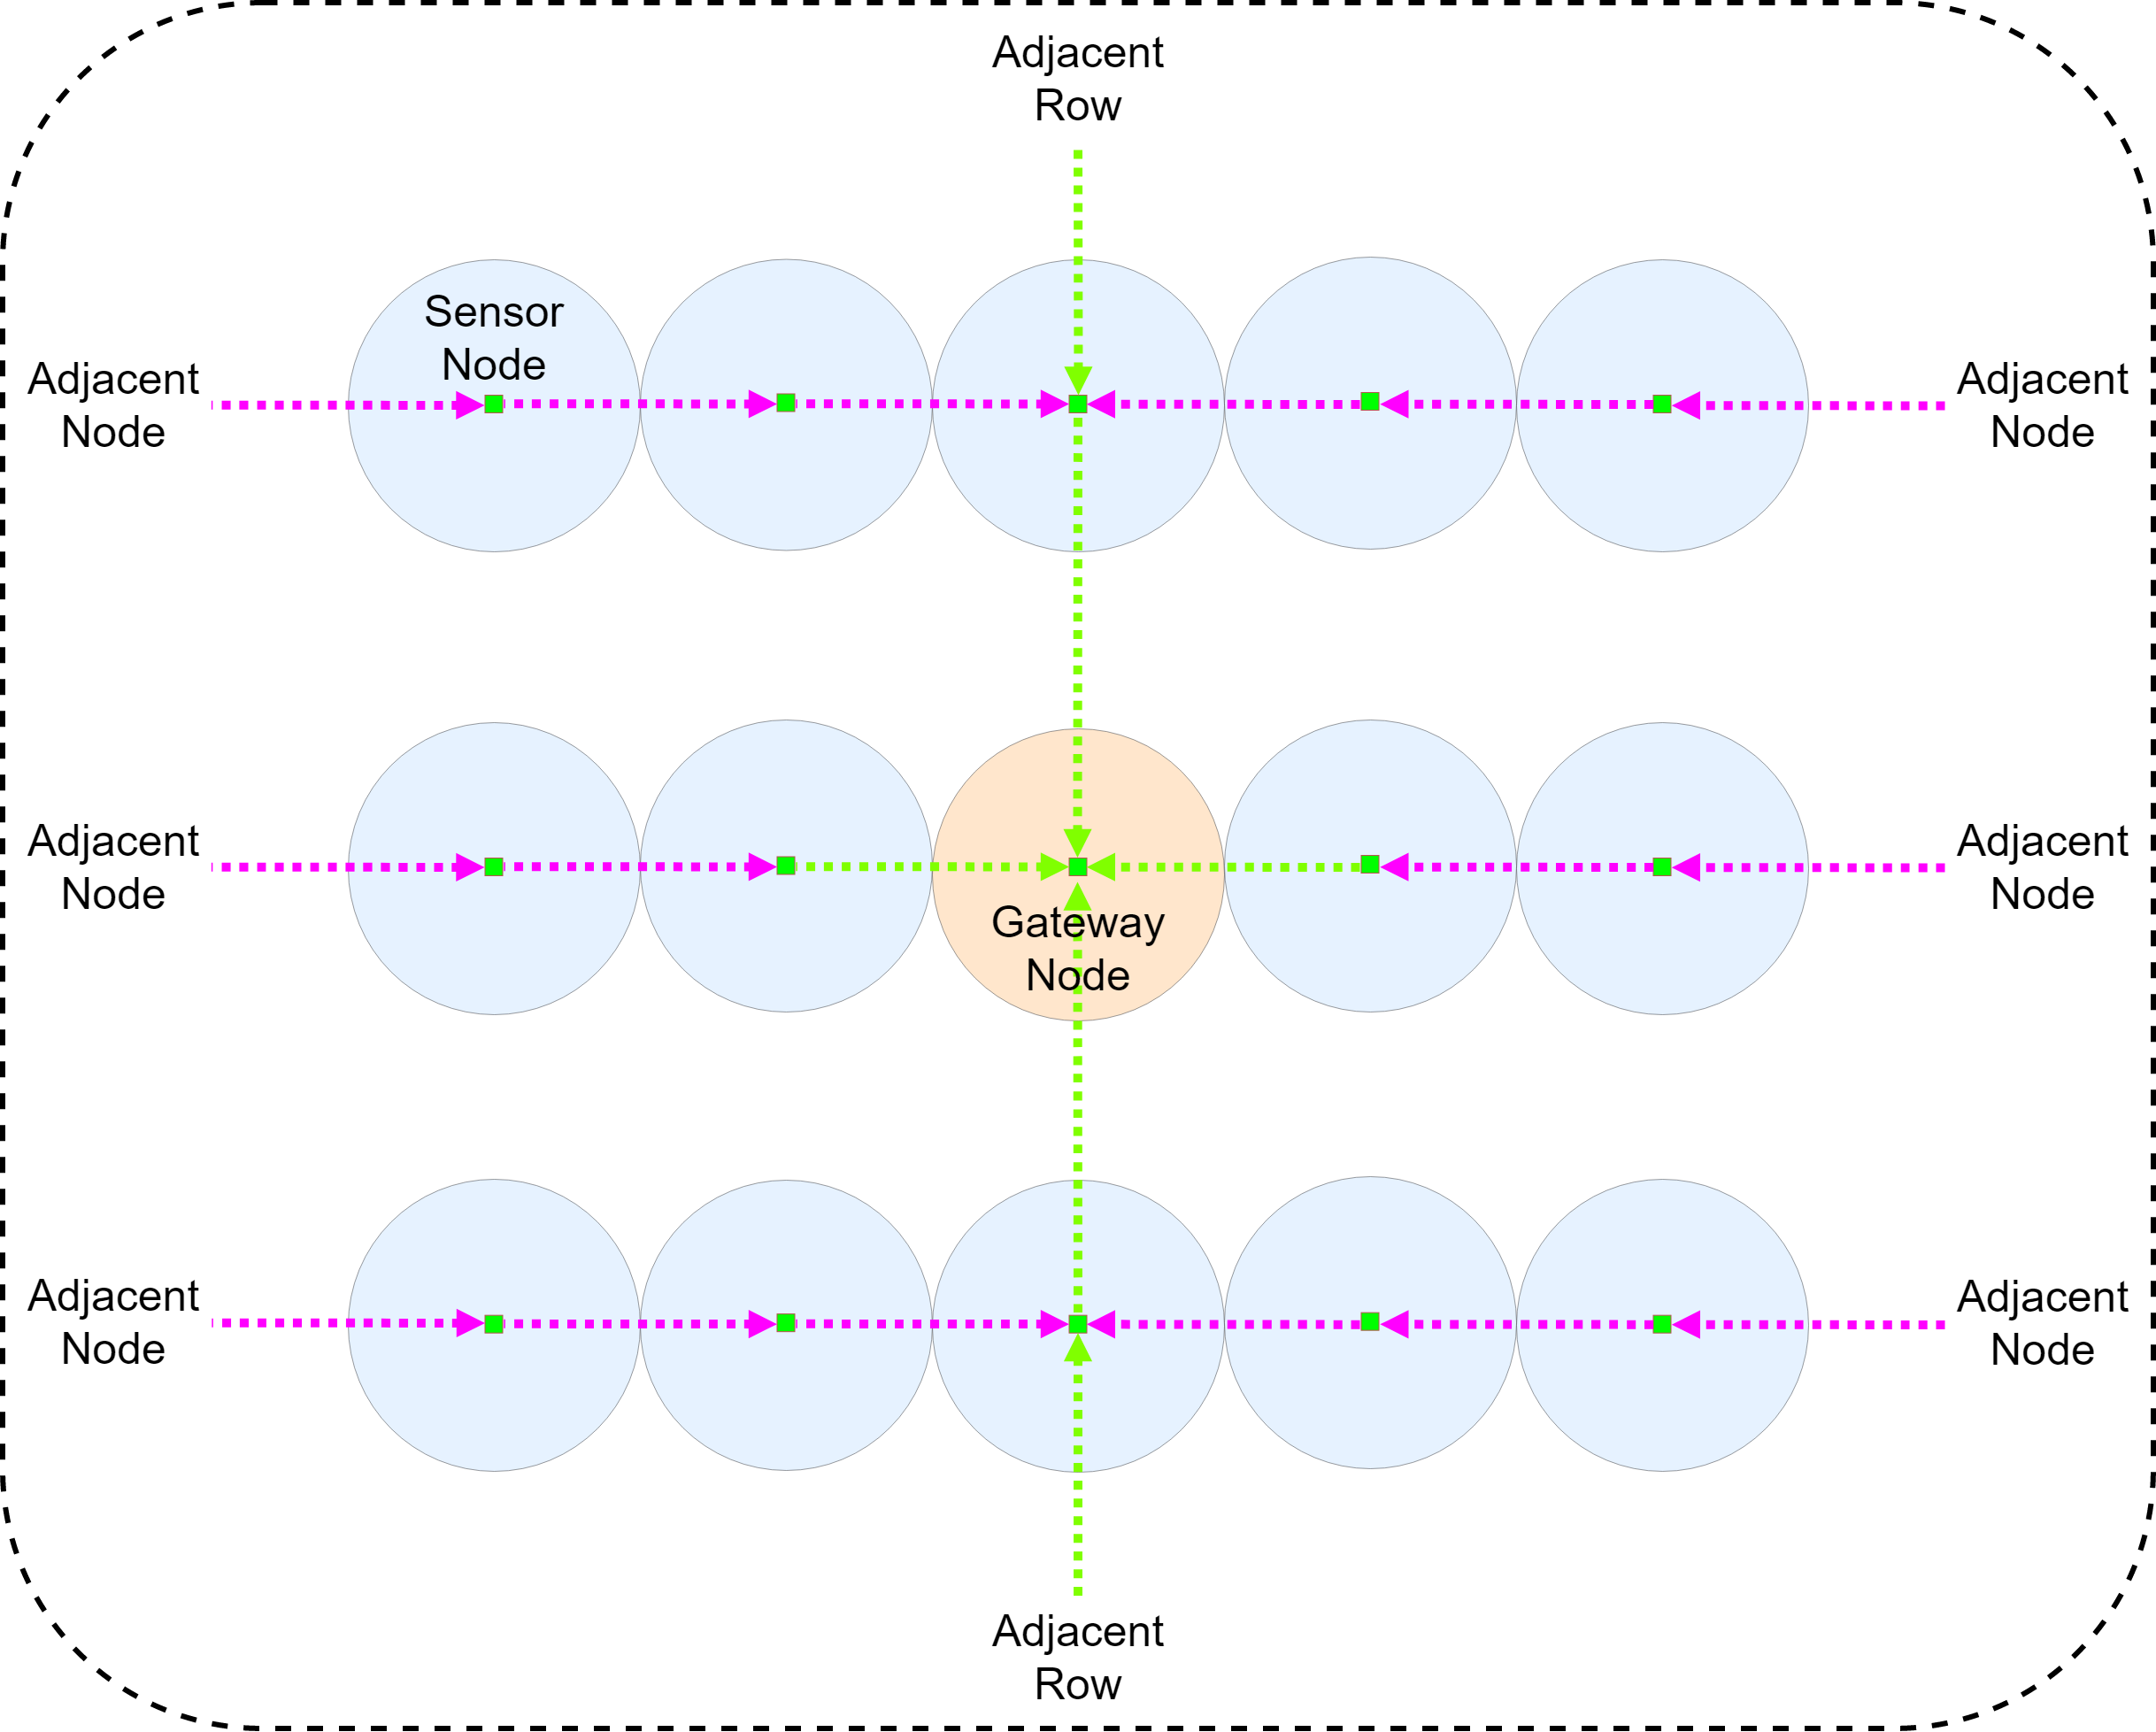
\includegraphics[width=1\columnwidth]{media/hop-mesh.png}
				\vspace{1em}
				\caption{Node network mesh which utilises single node hop communication for short range transmission}
				\raggedright
				\label{fig:single}
			\end{figure}
		
			\begin{figure}
				\centering
				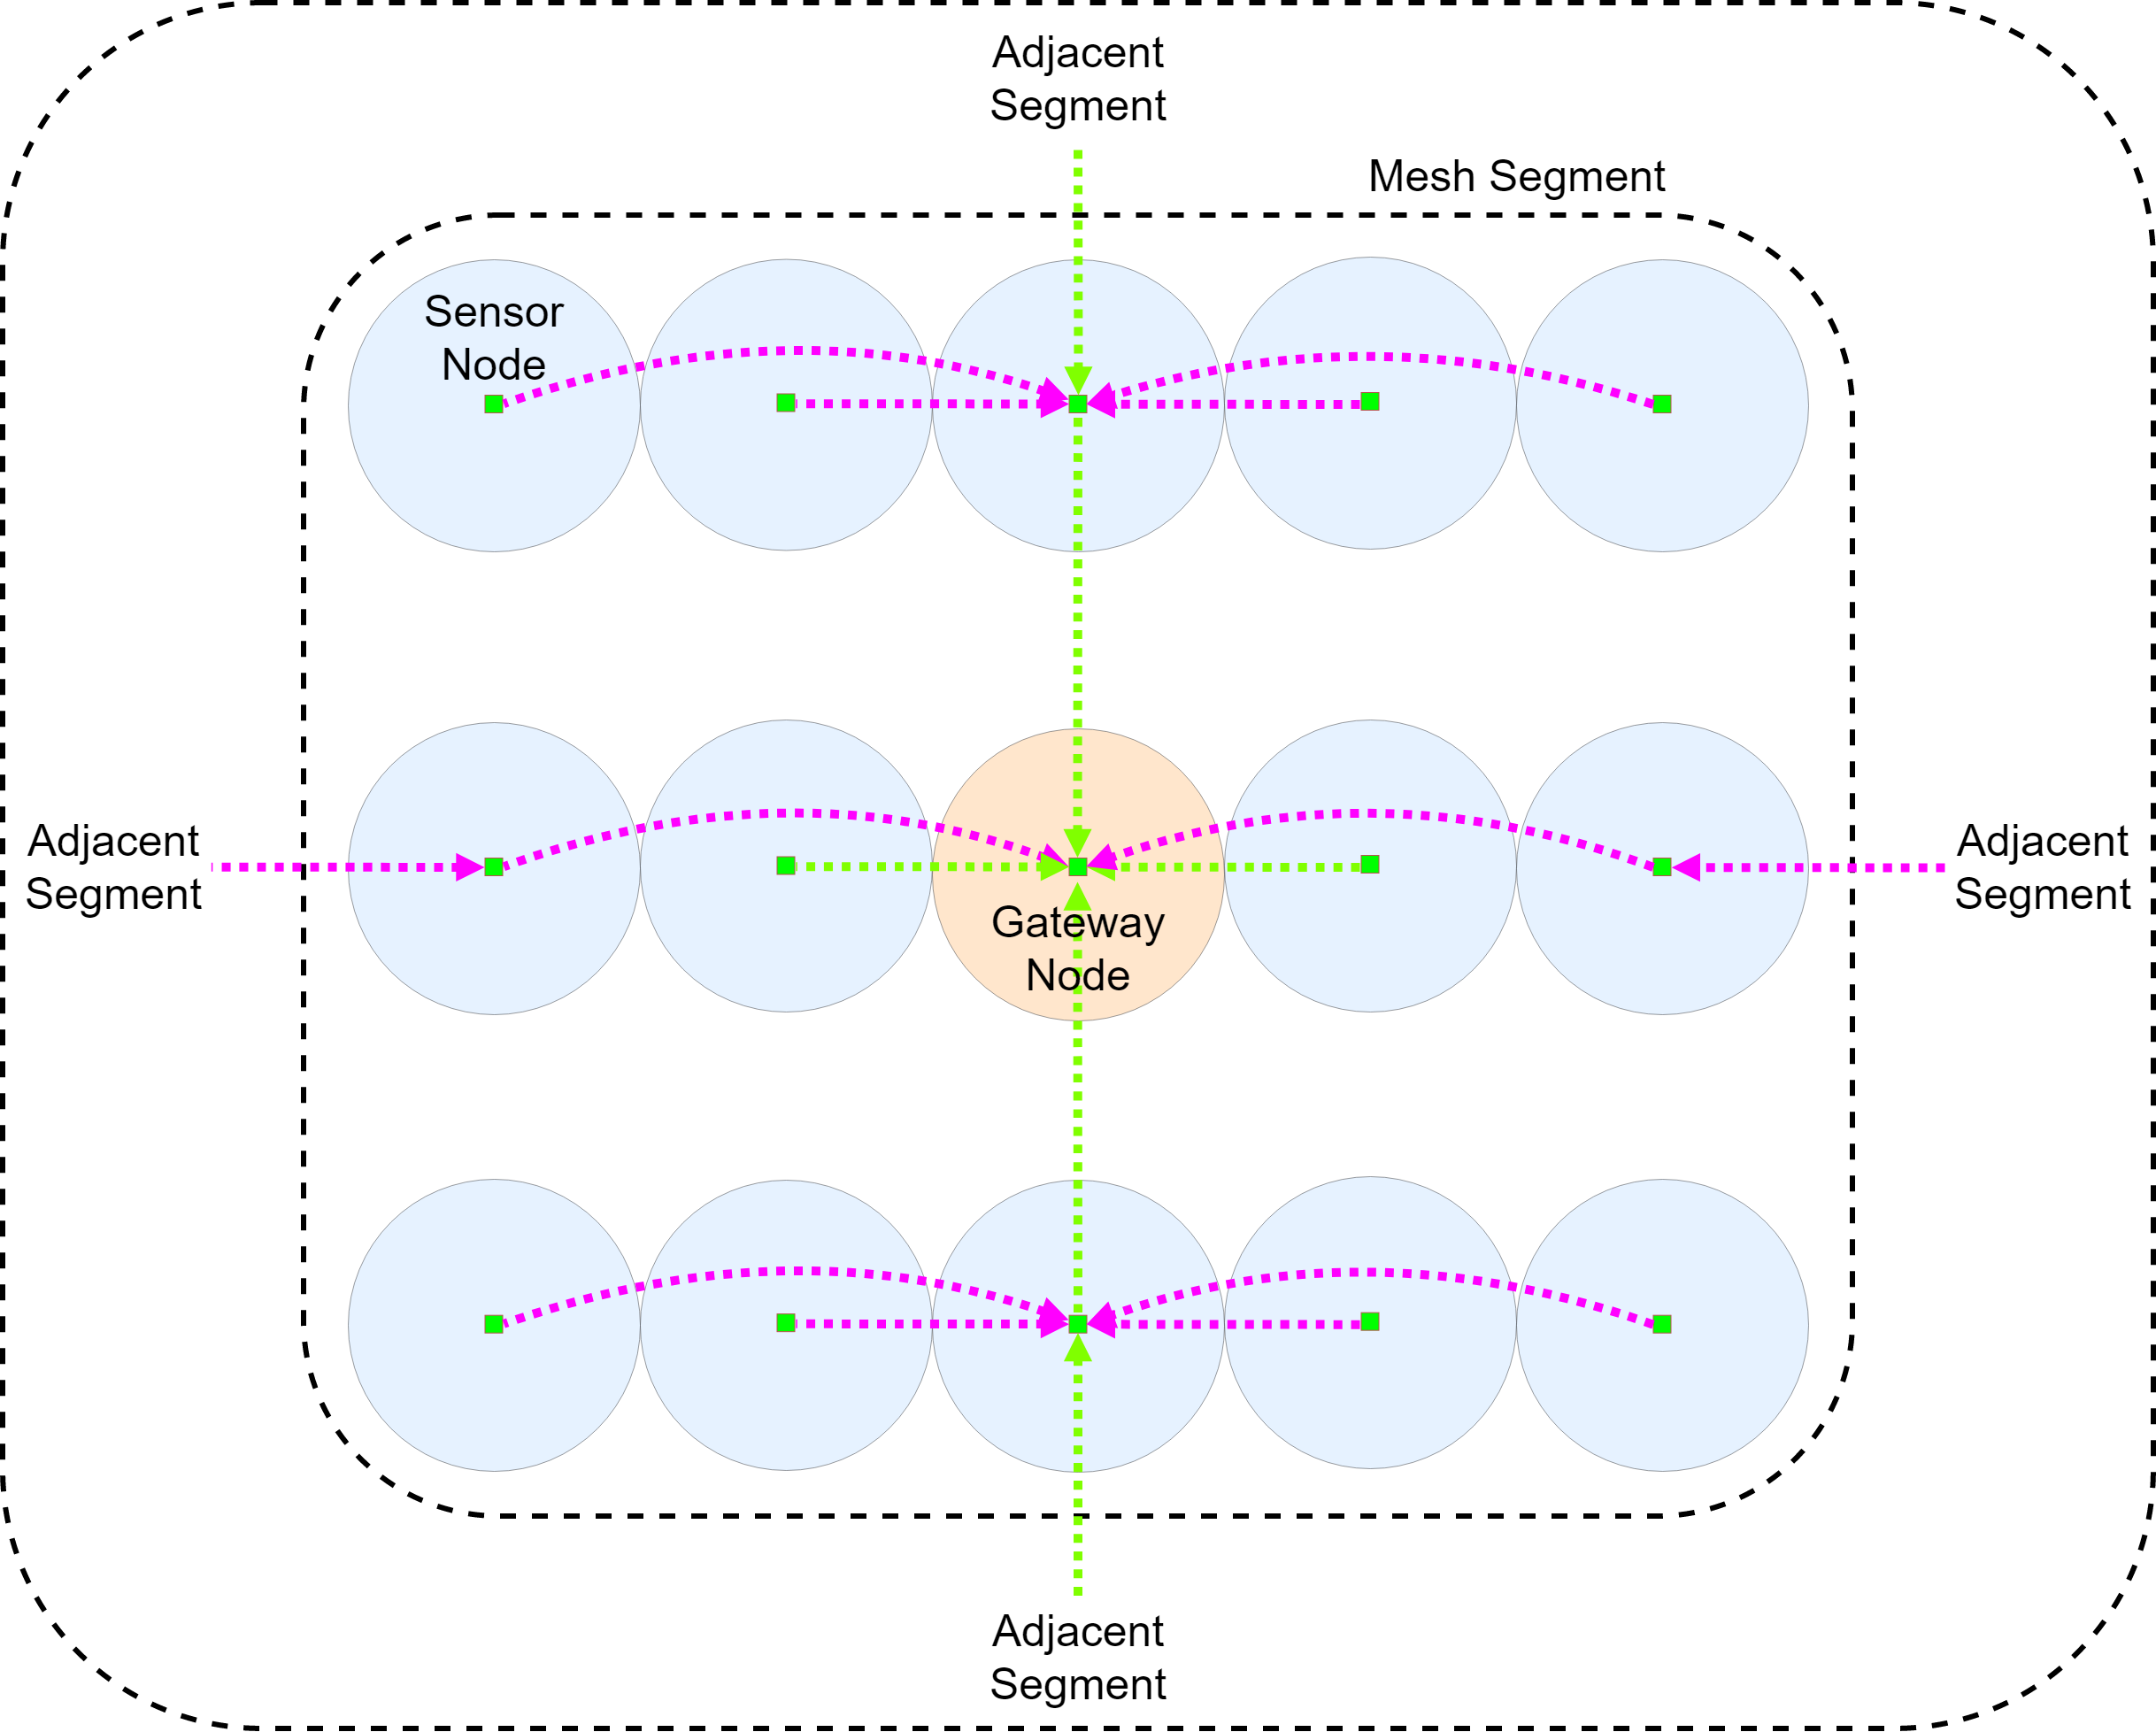
\includegraphics[width=1\columnwidth]{media/segment-mesh.png}
				\vspace{1em}
				\caption{Node network mesh which utilises multiple node hop communication in a segmented mesh configuration for longer range transmission with fewer hops}
				\raggedright
				\label{fig:segment}
			\end{figure}
	
		\subsubsection{Data Upload:}
			The Industrial, Scientific and Medical (ISM) band refers to a group of radio bands or parts of the radio spectrum that are unlicensed and internationally reserved for the use of RF energy intended for scientific, medical and industrial requirements. ISM bands are generally open frequency bands, which vary according to different regions and permits. Therefore any communication operating within the ISM band should be tolerant of interference from other ISM equipment. There has been a surge in low-power, short-range communication platforms utilising the ISM band such as bluetooth, Wi-Fi, NFC and mobile networks~\cite{ism}. Thus a large variety of communication methods are available offering a range of power consumptions, transmission ranges and data rates. The following communication methods are considered in uploading sensor data to the utilised data platform:
			
			\begin{itemize}
				
				\item GSM/GPRS:
				Global System for Mobile (GSM) communication, also commonly referred to as 2G, due to being a second-generation cellular network provides support for voice calls, Simple Message System (SMS) and data communication via General Packet Radio Service (GPRS). GPRS is a packet switching technology which can provide idealised data rates between 0.056~Mbps to 0.114~Mbps~\cite{gprs}. To utilise GPRS for data communication, an Access Point Name (APN) and username/passward pair is required from a network operator~\cite{gprs}.\\
				
				GSM modules are commercially available which are compatible with most major development boards. These modules require a Subscriber Identification Module (SIM) which is an integrated circuit with the purpose of securely storing the International Mobile Subscriber Identity (IMSI) number with its corresponding authentication key~\cite{imsi}. These are used to identify and authenticate subscribers on the mobile network. Such an example of a GSM module is the common Quectel M10 module which is a quad-band GSM/GPRS modem requiring a supply of just 3.4~V~\cite{m10}.\\

				\item Wits Wi-Fi:
				The university of the Witwatersrand (Wits) offers a high speed network, offering local and international data rates of 10~Gbps and 589~Mbps respectively~\cite{wits-speed}. Due to the constant need for connection on the main campus, the network is extremely reliable with minimal down-time.\\
				
				The use of a development board such as the ESP12-E which features a built in Wi-Fi module could easily be used as a gateway node for sensor network which could periodically collect all respective sensor data and thereafter connect to the Wi-Fi network provided by Wits to upload the sensor data to the utilised data platform~\cite{esp12e}.\\
			
				\item 4G:
				This is the fourth generation of broadband cellular network technology, succeeding 3G. This generation places emphasis on data rates. This is demonstrated in modules such as the Quectel EC25 LTE category 4 module which offers download and upload data rates of up to 150~mbps and 50~mbps respectively, requiring a supply of just 5~V~\cite{ec25}. This caters for solutions where large amounts of data needs to be transferred continuously.

			\end{itemize}

		\subsubsection{Data Platform}
			\begin{itemize}
				\item Amazon Web Services
				\item Google Cloud Platform
				\item Azure Web Services
				\item Thingspeak
				\item SigFox
				% max 12 byte payload
				% 6 uplinks/hour and 4 downlinks/day
			\end{itemize}
	
	\subsection{Data Presentation}
		\subsubsection{API}
		\subsubsection{User Interface}
			\begin{itemize}
				\item Web Application
				\item Mobile Application
			\end{itemize}

\section{PROJECT DESIGN}
	\subsection{Hardware Choices}
	%https://www.electronics-tutorials.ws/transistor/tran_4.html - may be useful
	
		% ref to circuit disgram in this section
		For the sensor nodes a combination of hardware choices have been made. The chosen MCU, an Arduino Nano V3, is powered by two rechargeable AA 12 V 3800mAh Ni-Mh batteries in series, boosted to 5V using a small boost converter, more commonly known as a step-up converter, circuit module. The 5V supply rail is also responsible for powering the four HCSR04 Ultrasonic Sensors attached to each module. The MCU will be responsible not only for deciding when and for how long the sensors should be powered (using a MOSFET transistor as a switch due to it's low voltage drop) but also to trigger their ultrasonic pulse for distance detection via the return echo signal. This will be achieved through the software configuration in an attempt to reduce power consumption and in turn extend the life of each module before a recharge is required. 
		
		The final component of each sensor node is the communication module, the NRF24L01+ transceiver. This module, powered by the 3.3V rail of the Arduino, transmits the sensor data over the mesh network to the access point, where all sensor data is combined and transmitted to the cloud via SigFox. The central node/access point consists of this SigFox module interfaced by an Arduino Uno board, powered similarly to that of the Nano modules mentioned above. The proposed circuit design is illustrated in \cref{fig:node-circuit}.

		\begin{figure*}[h]
			\centering
			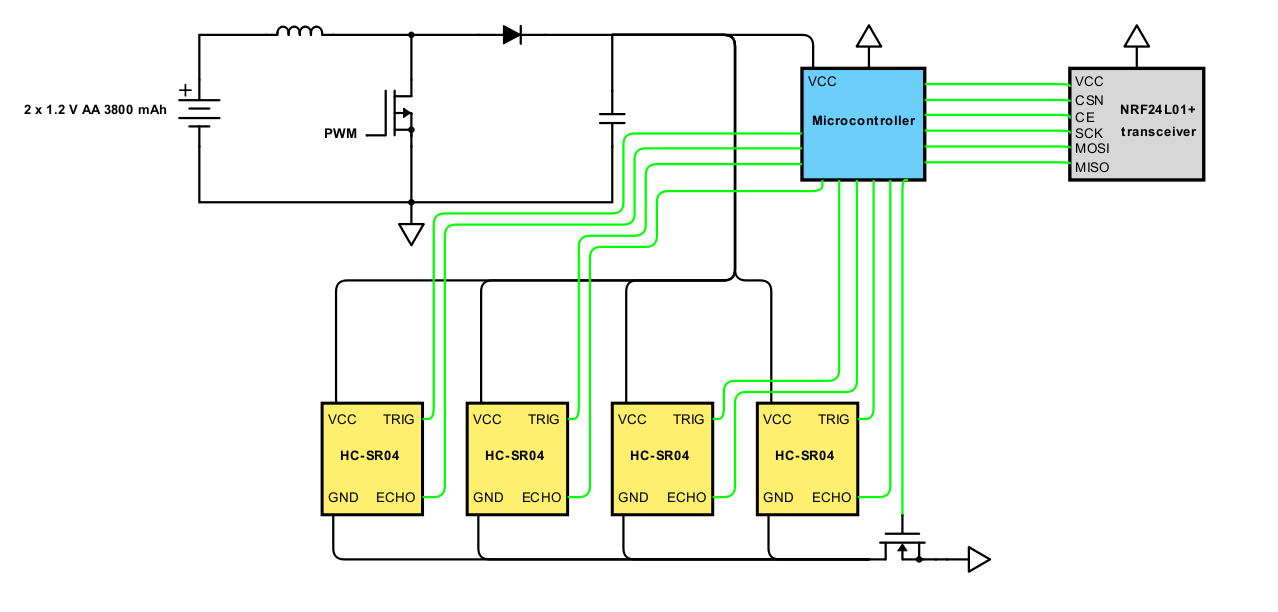
\includegraphics[width=\textwidth]{media/node-circuit.png}
			\caption{Circuit design of sensor node unit containing boost converter, MCU, ultrasonic sensors, and NRF24 transceiver}
			\raggedright
			\label{fig:node-circuit}
		\end{figure*}
	
	\subsection{Communication Technologies}
		The NRF24L01+ transceiver makes use of NRF24 RF technology to transmit data in the free 2.4GHz Industrial, Scientific and Medical (ISM) band. Each transceiver is capable of using 125 different channels in this band~\cite{howToMech_NRF24L01Tutorial}. The module can operate at a range of baud rates, where lower transfer rates increase its range. The achievable range is high but can be decreased with a decrease in transmission amplification power. The modules operate best in open air. To achieve this the devices should be configured such that data is transferred through as few obstacles as possible. 
		
		%SigFox or alternative, maybe use the ESP at the main node to transfer via wits wifi if we can't get enough info through often enough with SigFox
	
	\subsection{Deployment Methodologies}
		The sensor nodes will be deployed in a rigid encasing raised off the ground to average bumper height. The rigid encasing will most likely take form as an inexpensive yet rigid plastic encasing. This encasing will have the required windows for the ultrasonic sensors which will need to be recessed from the window. In turn all circuitry will be raised off the bottom of the encasing and drainage holes will be drilled on the underside to enable drainage if water is to enter via the windows.
		
		To raise the casing off the ground, a PVC stand will be assembled from electrical PVC conduits. The base will be held together by a 4 way PVC round box with four balance legs for stability. A vertical pole will be erected from the center of the stand on which the encased sensor node will be attached.
	
	\subsection{Data Management}

	\subsubsection{Data Platform}

	\subsection{Data Presentation}
		The process of translating raw sensor data into useful information occurs within the data presentation element of the designed solution. This will be served through a mobile application which is to be developed on the Android platform. The application will provide users, being students who wish to search for available parking spots, with a graphical user interface (GUI) in which an aerial view of the surveyed parking bays will be presented. An available parking by will be highlighted in green, whilst an occupied parking bay will be highlighted in red.

		The required sensor data will be obtained from the utilised data platform in the form of a RESTful application programming interface (API) which will allow the application to obtain the sensor data through hypertext protocol (HTTP) requests. The updated sensor data will be periodically requested by the application to provide regular GUI updates of available parking bays.
	
\section{PROJECT TESTING}
	\subsection{Testing Methodologies}


\section{PROJECT MANAGEMENT}

	Management of the project includes the management of work, time-management and scheduling, and the assessment and management of risks that are expected to be encountered throughout the project. The project can be divided into distinct phases in which specific workflow should take place.
	
	\subsection{Design Phase}
		The design phase consists of a series of iterations of ideation, feasibility analysis, refinement and critical analysis. An important part of the design phase is research, most of which has been presented in the early sections of this report. The final design should ideally be complete before the beginning of the project, yet realistically will continue throughout the implementation and testing phases. 
		
		Both the hardware and software components of the design must be considered here, to the point that all possible design implementations are known and the outcomes can be predicted with reasonable accuracy. 
	
	\subsection{Implementation Phase}
		The implementation phase will start once all hardware components have arrived and the design is finalised. Implementation will begin with the assembly of the sensor nodes as well as their programming. Following this the communication within the mesh network will be set up and tested. Once all sensor data is successfully retrieved by the access point, the data will be transmitted, via the SigFox module, to the SigFox cloud. From here a user application will be developed which can retrieve the parking availability data using an available API and presented to the user via an intuitive user interface.
	
	\subsection{Testing Phase}
		Testing will occur throughout the implementation phase. All individual modules, their collaboration, communications and accuracy will be verified as the system is put together. Once the finalised system is deployed into the parking lot, the system success rate will be tested using a statistical approach. Adjustments to improve the system accuracy will be made and iteratively, a low variance final product will be produced at the end of this phase.
		
	\subsection{Demonstration Phase}
		Demonstration is set to take place at Open Day. This phase involves creating posters as well as having the system deployed in the parking lot while the developed application demonstrates the system working in real time at the stand.
	
	\subsection{Documentation Phase}
		The final report is to be written and submitted during this phase. Although documentation will take place throughout all of the previous stages, writing the report is the sole focus of this phase.
	
	\subsection{Presentation Phase}
		The required final presentation is prepared in this phase. It is to be presented to the board of examiners once the final report has been submitted.
	
	\subsection{Projected Timeline}
	% look at project spec and flesh it out
	% we should probably discuss the real serious timeline like what people will have in Gannt charts somewhere. Seems like a good idea
	Figure~\ref{fig:timeline} demonstrates the projected project timeline and the phase progression for the project.
	
	\begin{figure}
		\centering
		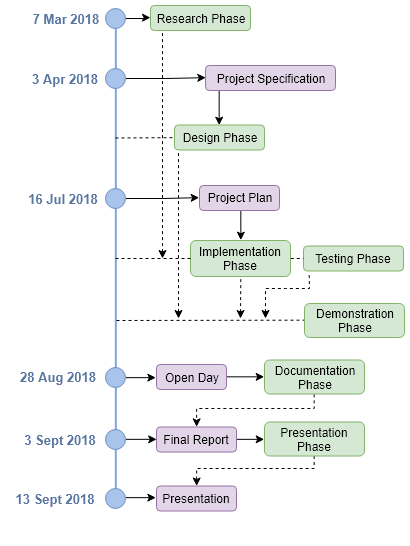
\includegraphics[width=1\columnwidth]{media/timeline.png}
		\caption{Projected timeline of the project, including workflow (green) and deadlines (purple)}
		\raggedright
		\label{fig:timeline}
	\end{figure}
	
	
	\subsection{Risk Assessment}
	% look at project spec and flesh it out

\section{CONCLUSION}

\bibliography{references}{}
\bibliographystyle{witseie}

\end{document}